\chapter{Ανάλογα ποσά - Αντιστρόφως ανάλογα ποσά}
\begin{exercise}
Να σχεδιάσεις ένα ορθοκανονικό σύστημα ημιαξόνων, με μονάδα το 1 cm και να
τοποθετήσεις τα σημεία Α(2,3), Β(3,2), Γ(4,5), Δ(5,5), Ε(1,4), Z(7,3), Η(7,2), Θ(6,2),
Ι(6,0), Κ(0,5). Τι παρατηρείς για τα σημεία Ι και Κ; Πού βρίσκονται αυτά; Μπορείς να
γενικεύσεις τις παρατηρήσεις σου για τα σημεία που έχουν τετμημένη ή τεταγμένη το
μηδέν;
\end{exercise}
\begin{lstlisting}
import matplotlib.pyplot as plt

plt.clf()
points = [(2,3), (3,2), (4,5), (5,5), (1,4), (7,3), (7,2), (6,2), (6,0), (0,5)]
pointName = ['Α','Β','Γ','Δ','Δ','Ε','Ζ','Η','Θ','Ι','Κ']
x = [p[0] for p in points]
y = [p[1] for p in points]
color=['m','g','r','b']
plt.grid()
plt.scatter(x,y, s=100 ,marker='o', c=color)
for (i,p) in enumerate(points):
    plt.annotate(pointName[i],(p[0],p[1]))

plt.show()
\end{lstlisting}
\begin{figure}
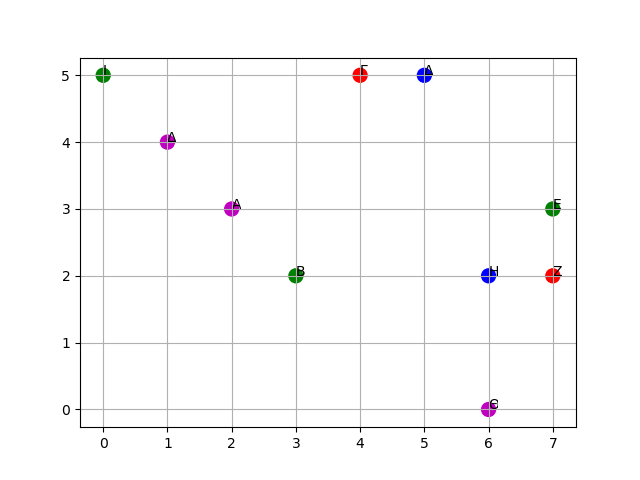
\includegraphics{graph1.png}
\end{figure}
\begin{exercise}
\sel[2]{89}
Σε ορθοκανονικό σύστημα ημιαξόνων να τοποθετήσεις τα σημεία Α(2,1), Β(1,2), Γ(2,3)
και Δ(3,2). Τι σχήμα είναι το ΑΒΓΔ; Αν τα ευθύγραμμα τμήματα ΑΓ και ΒΔ τέμνονται
στο σημείο Κ, ποιες είναι οι συντεταγμένες του Κ;
\end{exercise}
\begin{lstlisting}
import matplotlib.pyplot as plt

plt.clf()
points = [(2,1), (1,2), (2,3), (3,2)]
pointName = ['Α','Β','Γ','Δ']
x = [p[0] for p in points]
y = [p[1] for p in points]
color=['m','g','r','b']
plt.grid()
plt.scatter(x,y, s=100 ,marker='o', c=color)
for (i,p) in enumerate(points):
    plt.annotate(pointName[i],(p[0],p[1]))

x = [points[0][0],points[2][0]]
y = [points[0][1],points[2][1]]
plt.plot(x,y)
x = [points[1][0],points[3][0]]
y = [points[3][1],points[3][1]]
plt.plot(x,y)

plt.show()
\end{lstlisting}
\begin{figure}
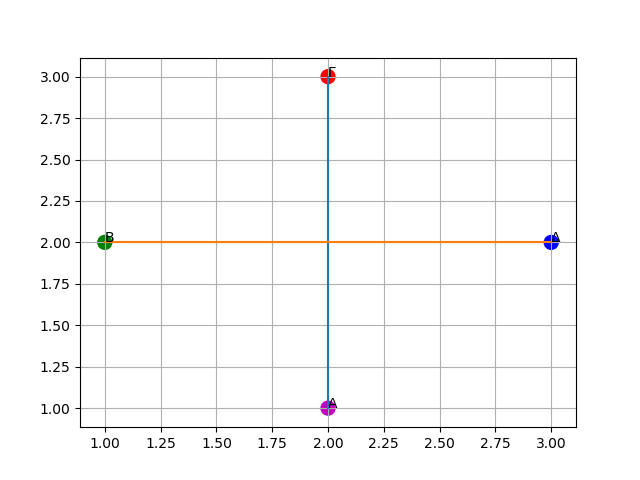
\includegraphics{graph2.png}
\end{figure}

\begin{exercise}
\sel[3]{89}
Γράψε πέντε διατεταγμένα ζεύγη σημείων, των οποίων η τετμημένη τους είναι ίση με
την τεταγμένη τους. Μπορείς να τα
τοποθετήσεις, σε ένα ορθοκανονικό
σύστημα ημιαξόνων; Τι παρατηρείς;
\end{exercise}
\begin{lstlisting}
import matplotlib.pyplot as plt

plt.clf()
points = [(1,1), (2,2), (5,5), (10,10), (15,15)]
pointName = ['Α','Β','Γ','Δ','Ε']
x = [p[0] for p in points]
y = [p[1] for p in points]
color=['m','g','r','b']
plt.grid()
plt.scatter(x,y, s=100 ,marker='o', c=color)
for (i,p) in enumerate(points):
    plt.annotate(pointName[i],(p[0],p[1]))

plt.show()
\end{lstlisting}
\begin{figure}
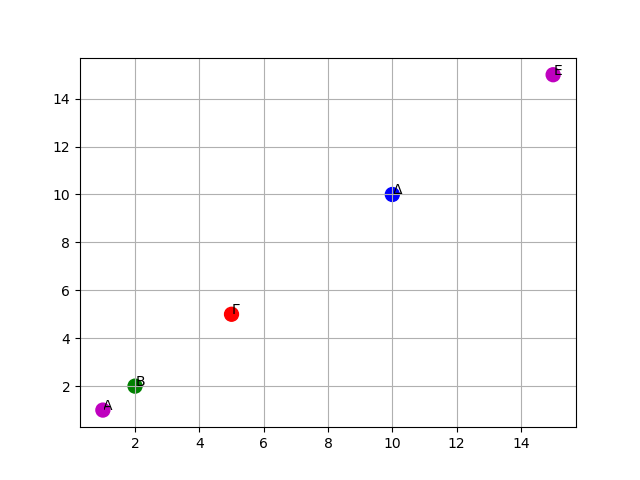
\includegraphics{graph3.png}
\end{figure}

\begin{exercise}
\sel{90}
Συμπλήρωσε τον παρακάτω πίνακα:
\begin{table}
\begin{tabular}{|l|c|c|c|}
Πλευρά τετραγώνου& 1,5 cm& 4 cm& 4,5 cm\\\hline
Περίμετρος τετραγώνου&&&\\\hline
\end{tabular}
\end{table}
\begin{itemize}
\item Εξήγησε πώς προκύπτουν οι αριθμοί της δεύτερης σειράς.
\item Βρες για κάθε τετράγωνο το κλάσμα πλευρά προς περίμετρο.
\item Ποιο είναι το συμπέρασμα που βγάζεις;
\end{itemize}
\end{exercise}
\begin{lstlisting}
>>> 4*1.5
6.0
>>> 4*4
16
>>> 4*4.5
18.0
\end{lstlisting}
\begin{tabular}{|l|c|c|c|}
Πλευρά τετραγώνου& 1,5 cm& 4 cm& 4,5 cm\\\hline
Περίμετρος τετραγώνου&6&16&18\\\hline
\end{tabular}
Θυμηθείτε το ποσοστό σε κλάσμα:
\begin{lstlisting}
def posostoseklasma(fx):
    fx = float(fx)
    denom = 100
    while int(fx) != fx:
         fx *= 10
         denom *= 10
    fx = int(fx)
    return(Fraction(fx,denom))
\end{lstlisting}
Το fx είναι είναι ο αριθμητής ενός κλάσματος με παρονομαστή 100. Εδώ δεν θα υπάρχει ο παρονομαστής 100 οπότε έχουμε denom = 1.
\begin{lstlisting}
def dekadikosseklasma(fx):
    fx = float(fx)
    denom = 1
    while int(fx) != fx:
         fx *= 10
         denom *= 10
    fx = int(fx)
    return(Fraction(fx,denom))

dekadikosseklasma(1.5/6)
dekadikosseklasma(4/16)
dekadikosseklasma(4.5/18)
\end{lstlisting}
και το αποτέλεσμα είναι:
\begin{lstlisting}
>>> dekadikosseklasma(1.5/6)
Fraction(1, 4)
>>> dekadikosseklasma(4/16)
Fraction(1, 4)
>>> dekadikosseklasma(4.5/18)
Fraction(1, 4)
\end{lstlisting}
Άρα παντού το κλάσμα είναι $\frac{1}{4}$.
\begin{exercise}
\sel{90}
Χρησιμοποιούμε τη φωτογραφική μηχανή
για να απεικονίσουμε εικόνες αντικειμένων. Οι εικόνες αυτές δείχνουν τα
πραγματικά αντικείμενα σε σμίκρυνση.
Στη φωτογραφία το ύψος ενός παιδιού
είναι 2 cm ενώ γνωρίζουμε ότι το πραγματικό του ύψος είναι 1,65 m = 165 cm. Πόση θα είναι τότε η σμίκρυνσή του
στη φωτογραφία;
\end{exercise}
\begin{lstlisting}
>>> 2/165
0.012121212121212121
\end{lstlisting}

\begin{exercise}
\sel{91}
Μετρούμε μια απόσταση, σε χάρτη, με κλίμακα 1:10.000.000 και τη βρίσκουμε
ίση με 2,4 cm. Ποια είναι η πραγματική απόσταση των δύο σημείων;
\end{exercise}
\begin{lstlisting}
>>> x = 2.4*10000000
>>> x
24000000
>>> x = x/100
>>> x
240000
>>> x = x/1000
>>> x
240
\end{lstlisting}
240Km
\begin{exercise}
\sel[3]{92}
Σε μια φωτογραφία το ύψος ενός ανθρώπου είναι 4 cm, ενώ το
πραγματικό το ύψος είναι 1,76 m. Πόσο έχει σμικρυνθεί η εικόνα του
ανθρώπου στη φωτογραφία;
\end{exercise}
\begin{lstlisting}
def pososto(x):
    print(str(round(x*100,2))+'%')
\end{lstlisting}
Αν θυμηθούμε τη συνάρτηση pososto τότε
\begin{lstlisting}
>>> pososto(4/176)
2.27%
\end{lstlisting}
\begin{exercise}
\sel[4]{92}Ένας προβολέας διαφανειών προβάλλει το κείμενο μιας διαφάνειας στον απέναντι
τοίχο. Αν ένα ``A'' έχει ύψος 7 mm στη διαφάνεια και 4,2 cm στον τοίχο, ποια είναι η
μεγέθυνση που δίνει ο προβολέας
\end{exercise}
\begin{lstlisting}
>>> pososto(4.2/0.7)
600%
\end{lstlisting}
\begin{exercise}
\sel[5]{92}
Η σύνθεση μιας μπλούζας είναι 80\% βαμβάκι και το υπόλοιπο πολυεστέρας. Aν η μπλούζα
ζυγίζει 820 gr, πόσα γραμμάρια ζυγίζουν τα νήματα του πολυεστέρα που περιέχει;
\end{exercise}
\begin{lstlisting}
>>> 820*20/100
164.0
\end{lstlisting}
\begin{exercise}
\sel[6]{92}
Να συμπληρωθεί ο πίνακας
\begin{table}
\begin{tabular}{|c|c|c|c|c|c|}
\hline
Κλίμακα&1:5&3:8&1:30&&1:100\\\hline
Μήκος σε σχέδιο&4cm &&12cm&2cm&3,5cm\\\hline
Πραγματικό ύψος&&24m&&10m&\\\hline
\end{tabular}
\end{table}
\end{exercise}
\begin{lstlisting}
>>> from fractions import Fraction
>>> 5*4
20
>>> 3/8*24
9.0
>>> 12*30
360
>>> Fraction(2,1000)
Fraction(1, 500)
>>> 3.5*100
350
\end{lstlisting}
Άρα ο πίνακας γίνεται:
\begin{table}
\begin{tabular}{|c|c|c|c|c|c|}
\hline
Κλίμακα&1:5&3:8&1:30&1:500&1:100\\\hline
Μήκος σε σχέδιο&4cm &9cm&12cm&2cm&3,5cm\\\hline
Πραγματικό ύψος&20cm&24m&360cm&10m&350cm\\\hline
\end{tabular}
\end{table}
\begin{exercise}
\sel[7]{92}
Οι διαστάσεις ενός ορθογωνίου παραλληλογράμμου είναι $x+2$ και $x$.

(α) Να γράψεις τη σχέση που συνδέει την περίμετρο Π του ορθογωνίου με το x.

(β) Να συμπληρώσεις τον πίνακα:
\begin{table}
\begin{tabular}{|c|c|c|c|c|}
x&&2&&4\\\hline
Π&8&&16&\\\hline
\end{tabular}
\end{table}
\end{exercise}
α)
\begin{lstlisting}
>>> from sympy import *
>>> x = symbols('x')
>>> p = x+x+2+x+x+2
>>> p
4*x + 4
\end{lstlisting}
β)
\begin{lstlisting}
>>> solve(p-8)
[1]
>>> p.subs(x,2)
12
>>> solve(p-16)
[3]
>>> p.subs(x,4)
20
\end{lstlisting}
και ο πίνακας γίνεται:
\begin{table}
\begin{tabular}{|c|c|c|c|c|}
\hline
x&1 &2  &3  &4\\\hline
Π&8&12&16&20\\\hline
\end{tabular}
\end{table}
\begin{exercise}
\sel[8]{92}
Aν οι διαστάσεις ενός δωματίου, σε ένα σχέδιο με κλίμακα 1:250, είναι 3x5, οι
πραγματικές διαστάσεις του δωματίου θα είναι .....x..... .
\end{exercise}
\begin{lstlisting}
>>> 3*250
750
>>> 5*250
1250
\end{lstlisting}
Οπότε το δωμάτιο είναι 7,5m x 12,5m αν οι διαστάσεις ήταν σε cm.
\begin{exercise}
\sel[9]{92}
Αν ανακατέψουμε 2 κιλά κόκκινο χρώμα και 3 κιλά κίτρινο χρώμα,
φτιάχνουμε μια συγκεκριμένη απόχρωση του πορτοκαλί. Αν
ανακατέψεις 5 κιλά κόκκινο χρώμα και 6 κιλά κίτρινο, θα πάρεις
την ίδια απόχρωση; Δικαιολόγησε την απάντησή σου.
\end{exercise}
\begin{lstlisting}
>>> 3/2 == 6/5
False
\end{lstlisting}
Όχι δεν είναι η ίδια απόχρωση.
\begin{exercise}
\sel[2]{93} Όταν ο Κώστας έκλεισε τα δώδεκα χρόνια είχε το ένα τρίτο της
ηλικίας της μητέρας του. Όταν θα γίνει είκοσι χρόνων, ο λόγος των
δύο ηλικιών τους θα παραμείνει ο ίδιος;
\end{exercise}
\begin{lstlisting}
>>> ilikiaMiteras = 3*12
>>> ilikiaMiteras
36
>>> xronia = 20-12
>>> xronia
8
>>> neailikiaMiteras = ilikiaMiteras + xronia
>>> neailikiaMiteras = 44
>>> 44/20 == 36/12
False
\end{lstlisting}
Άρα όχι.
\begin{exercise}
Να συμπληρωθεί ο πίνακας, αν γνωρίζουμε ότι τα ποσά x και 􀁜 είναι ανάλογα, με
συντελεστή αναλογίας $\alpha = \frac{2}{3}$.
\begin{table}
\begin{tabular}{|c|c|c|c|c|c|c}
\hline
x &0 &1 &0,3& &\\\hline
y &    &  &       & $\frac{5}{3}$ & 3\\\hline
\end{tabular}
\end{table}
\end{exercise}
$$
y = \frac{2}{3}x
$$
\begin{lstlisting}
>>> from sympy import *
>>> (x,y) = symbols('x y')
>>> e = 2/3*x
>>> e.subs(x,0)
0
>>> e.subs(x,1)
0.666666666666667
>>> e.subs(x,0.3)
0.200000000000000
>>> solve(e-5/3)
[2.50000000000000]
>>> solve(e-3)
[4.50000000000000]
\end{lstlisting}
Και ο πίνακας γίνεται:
\begin{table}
\begin{tabular}{|c|c|c|c|c|c|c}
\hline
x &0 &1 &0,3& 2,5&4,5\\\hline
y & 0   & 0,6666 & 0,2      & $\frac{5}{3}$ & 3\\\hline
\end{tabular}
\end{table}
\begin{exercise}
\sel[2]{92}
Σε ένα διάλυμα ζάχαρης η περιεκτικότητα σε ζάχαρη είναι 23\%. Πόσα γραμμάρια
ζάχαρης υπάρχουν σε 300 gr διαλύματος;
\end{exercise}
\begin{lstlisting}
>>> 300*23/100
69.0
\end{lstlisting}
\begin{exercise}
\sel[3]{97}
Ένα πλοίο έχει σταθερή ταχύτητα και καλύπτει απόσταση 80 Km σε 2 ώρες. Σε πόσο
χρόνο θα καλύψει απόσταση 2.000 Km;
\end{exercise}
$$\frac{2}{80}=\frac{x}{2000}$$
\begin{lstlisting}
>>> from sympy import *
>>> x = symbols('x')
>>> solve(2/80-x/2000)
[50.0000000000000]
\end{lstlisting}
Η απάντηση είναι 50 ώρες.
\begin{exercise}
Εξέτασε αν τα ποσά που δίνονται στους παρακάτω πίνακες είναι ανάλογα:
(α) 
\begin{table}
\begin{tabular}{|c|c|c|c|}
\hline
x&3&5 &7\\\hline
y&8&10&12\\\hline
\end{tabular}
\end{table}
(β)
\begin{table}
\begin{tabular}{|c|c|c|c|c|}
\hline
x&3&4 &6&11\\\hline
y&0,9&1,2&1,8&3,3\\\hline
\end{tabular}
\end{table}
\end{exercise}
\begin{lstlisting}
>>> 8/3==10/5==12/7
False
>>> 0.9/3==1.2/4==1.8/6==3.3/11
True
\end{lstlisting}
\begin{exercise}
\sel[4]{98}
Στον πίνακα που ακολουθεί, τα ποσά x και y είναι ανάλογα. Υπολόγισε τον συντελεστή
αναλογίας τους και συμπλήρωσε τον πίνακα.
\begin{table}
\begin{tabular}{|c|c|c|c|c|c|c|c|c|}
x& 5& 0& 1& & & 3,7& 0,61&\\\hline
y&10,05& & &2 &0,125&&& 0,55\\hline
\end{tabular}
\end{table}
\end{exercise}
Η αναλογία είναι 
\begin{lstlisting}
>>> 10.05/5
2.0100000000000002
\end{lstlisting}
Όμως αυτό είναι 2,01
Οπότε:
\begin{lstlisting}
>>> 0*2.01
0.0
>>> 1*2.01
2.01
>>> 2/2.01
0.9950248756218907
>>> 0.125/2.01
0.06218905472636817
>>> 3.7*2.01
7.436999999999999
>>> 0.61*2.01
1.2260999999999997
>>> 0.55/2.01
0.27363184079601993
\end{lstlisting}
και προσεγγιστικά ο πίνακας γίνεται:
\begin{table}
\begin{tabular}{|c|c|c|c|c|c|c|c|c|}
x& 5       & 0& 1      &0,995 & 0,0622 & 3,7   & 0,61&  0,273632\\\hline
y&10,05& 0 & 2.01&2         &0,125      &7,437& 1.226&0,55\\hline
\end{tabular}
\end{table}

\section{Ανάλογα ποσά}
\begin{exercise}
Σε	μια	παρέα	κάποιος	υποστήριζε	ότι	το	βάρος	του	ανθρώπου	είναι	ανάλογο	του	ύψους	του. Μετρήθηκαν,	λοιπόν,	όλοι	και	έβαλαν	στον	παρακάτω	πίνακα	τα	αποτελέσματα σε Κ.
\begin{table}
\begin{tabular}{|c|c|c|c|c|}
\hline
Βάρος& 58& 71& 56& 68\\\hline
Ύψος & 1,60&1,65&1,62&1,72\\\hline
\end{tabular}
\end{table}
\begin{itemize}
\item Μπορείς	να	επιβεβαιώσεις	ή	να	απορρίψεις	τον		ισχυρισμό	αυτό;		
\item Πώς	δικαιολογείς	το	συμπέρασμά	σου;
\end{itemize}
\end{exercise}
\begin{lstlisting}
>>> 58/1.60 == 71/1.65
False
\end{lstlisting}
Οπότε ο ισχυρισμός απορρίπτεται.
\begin{exercise}
O	μανάβης	πουλάει	τα	καρπούζια	προς	0,4	Q
	το	κιλό.	Μέσα	σε	μια	ημέρα	πούλησε	11	καρπούζια	που	ζύγιζαν	100	κιλά	συνολικά.	Ο	μανάβης	έγραφε,	σ’	ένα	χαρτί,	τα	λεφτά	που	 εισέπραττε	κάθε	φορά.	Ξέχασε,	όμως,	μία	φορά	να	το	σημειώσει.

→		Μπορείς	να	τον	βοηθήσεις	συμπληρώνοντας 	τα	κενά	του	παρακάτω	πίνακα: 
\begin{table}
\begin{tabular}{|c|c|c|c|c|c|c|c|c|c|c|c|}
\hline
Tιμή& 6€ & 2,8€ & 5,2€ & 3,2€ & & 3,6€ & 4,8€ & 2,4€ & 1,6€ & 4,4€ & 2€\\\hline
Κιλά&       &         &          &         &&            &          &          &        &            &     \\\hline
\end{tabular}
\end{table}    
\begin{itemize}
 \item Δικαιολόγησε τα	αποτελέσματα	των	πράξεων	που 	έκανες	και	προσπάθησε	να		διατυπώσεις	έναν	γενικό	κανόνα. 
\end{itemize}

 \end{exercise}
 Τα χρήματα που πήρε συνολικά θα είναι $0,4*100=40$€. Οπότε μπορούμε να αθροίσουμε τα χρήματα και να βρούμε τα κιλά που πωλήθηκαν από τα χρήματα.
 \begin{lstlisting}
 >>> 6+2.8+5.2+3.2+3.6+4.8+2.4+1.6+4.4+2
36.0
>>> 36/0.4
90.0
>>> 100-90
10
>>> 10*0.4
4.0
\end{lstlisting}
Για να συμπληρώσουμε ολόκληρο τον πίνακα μπορούμε να βρούμε τα κιλά από τα χρήματα διαιρώντας με το 0,4.
\begin{lstlisting}
>>> 6/0.4
15.0
>>> 2.8/0.4
6.999999999999999
>>> 5.2/0.4
13.0
>>> 3.6/0.4
9.0
>>> 4.8/0.4
11.999999999999998
>>> 2.4/0.4
5.999999999999999
>>> 1.6/0.4
4.0
>>> 4.4/0.4
11.0
>>> 2/0.4
5.0
>>>
\end{lstlisting}
Αν λάβουμε υπόψη τις στρογγυλοποιήσεις ο πίνακας γίνεται:
\begin{table}
\begin{tabular}{|c|c|c|c|c|c|c|c|c|c|c|c|}
\hline
Tιμή& 6€ & 2,8€ & 5,2€ & 3,2€ & 4€ & 3,6€ & 4,8€ & 2,4€ & 1,6€ & 4,4€ & 2€\\\hline
Κιλά&  15 &  7    &   13    &   8      & 10& 9      &  12    &   6     &  4    &   1       &  5   \\\hline
\end{tabular}
\end{table}    
\begin{exercise}
\sel{99}
Η	σχέση,	μεταξύ	δύο	ανάλογων	ποσών	x	και		με	συντελεστή	αναλογίας	α	=	3,	δίνεται	από	τον	τύπο:		
$$ y =	3 \cdot x$$.
\begin{itemize}
\item Συμπλήρωσε	τα	κενά	του	πίνακα	και	με	άλλες	τιμές	των	αναλόγων	ποσών	x	και	.
\item Βρες	τα	σημεία	του	επιπέδου	που		αναπαριστούν	τα	παραπάνω		ζεύγη	τιμών.
\item Προσπάθησε	να	διαπιστώσεις,	εάν		τα	σημεία	ανήκουν	σε	μία	ημιευθεία		ή	όχι.	
\item Η	ημιευθεία	αυτή	περνάει	από		το	σημείο	Ο(0,0)	δηλαδή	την	αρχή		των	ημιαξόνων;
\end{itemize}
\end{exercise}
\begin{lstlisting}
import matplotlib.pyplot as plt
from random import randint
from math import floor
plt.clf()
points = []
for i in range(10):
    x = 0+randint(0,10)*0.5
    y = 3*x
    points.append((x,y))

x = [p[0] for p in points]
y = [p[1] for p in points]
color=['m','g','r','b']
plt.grid()
plt.scatter(x,y, s=100 ,marker='o', c=color)

plt.show()
\end{lstlisting}
\begin{figure}
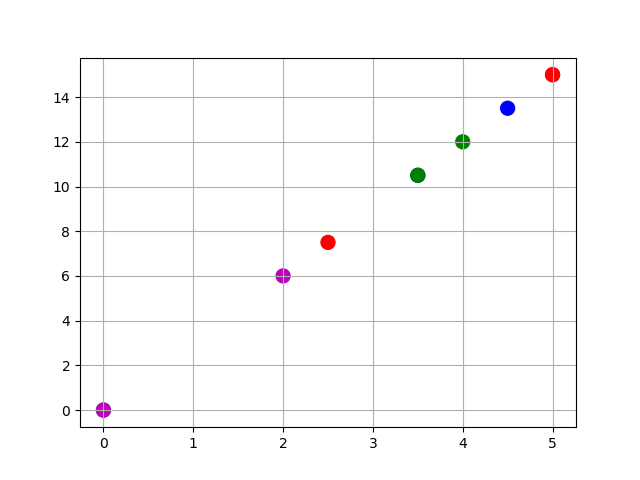
\includegraphics{3x.png}
\end{figure}
Οπότε τα σημεία ανήκουν σε ημιευθεία η οποία περνάει από την αρχή των αξόνων.

\begin{exercise}
\sel{100}
Δίνονται	οι	 πίνακες	Α,	Β,	 Γ	και	Δ.	

(α)	Να	γίνει	η	γραφική	απεικόνιση	των	ζευγών	(x,y)	των	πινάκων	στο επίπεδο	και	
(β)	να	διαπιστωθεί	σε	ποια	περίπτωση	αυτά	παριστάνουν	ποσά	ανάλογα.   

\begin{table}
\begin{tabular}{|c|c|c|c|c|}
x&0&1&2&3\\
y&0&2&1&1.5\\
\end{tabular}
\caption{Πίνακας Α}
\end{table}

\begin{table}
\begin{tabular}{|c|c|c|c|c|}
x&0&1&2&3\\
y&1&1.5&2&2.5\\
\end{tabular}
\caption{Πίνακας B}
\end{table}

\begin{table}
\begin{tabular}{|c|c|c|c|c|}
x&0&1&2&3\\
y&0&1&2&3\\
\end{tabular}
\caption{Πίνακας Γ}
\end{table}


\begin{table}
\begin{tabular}{|c|c|c|c|c|}
x&0&1&2&3\\
y&0&0.5&1&1.5\\
\end{tabular}
\caption{Πίνακας Δ}
\end{table}
\end{exercise}
\begin{lstlisting}
import matplotlib.pyplot as plt

plt.clf()
pointsA = [(0,0),(1,2),(2,1),(3,1.5)]
pointsB = [(0,1),(1,1.5),(2,2),(3,2.5)]
pointsC = [(0,0),(1,1),(2,2),(3,3)]
pointsD = [(0,0),(1,0.5),(2,1),(3,1.5)]

x = [p[0] for p in pointsA]
y = [p[1] for p in pointsA]
plt.grid()
plt.plot(x,y, marker='o', c='r')


x = [p[0] for p in pointsB]
y = [p[1] for p in pointsB]
plt.grid()
plt.plot(x,y, marker='o', c='g')


x = [p[0] for p in pointsC]
y = [p[1] for p in pointsC]
plt.grid()
plt.plot(x,y,marker='o', c='b')


x = [p[0] for p in pointsD]
y = [p[1] for p in pointsD]
plt.grid()
plt.plot(x,y, marker='o', c='m')
plt.show()
\end{lstlisting}

\begin{figure}
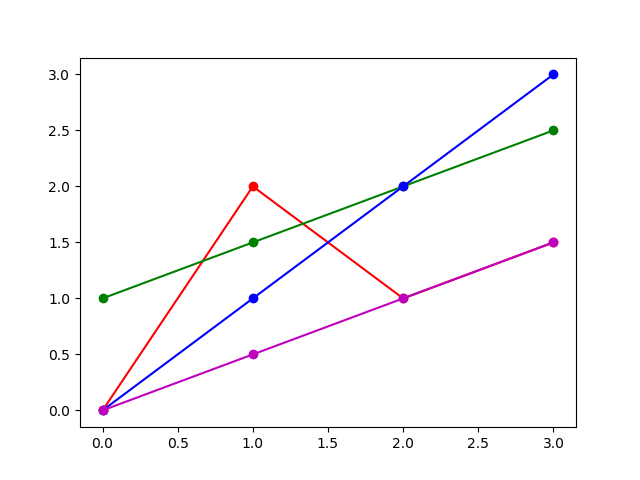
\includegraphics{4plots.png}
\end{figure}

Μια πιο σύντομη έκδοση του προγράμματος που δίνει το ίδιο αποτέλεσμα είναι:
\begin{lstlisting}
import matplotlib.pyplot as plt

plt.clf()
pointslist = [[(0,0),(1,2),(2,1),(3,1.5)],
          [(0,1),(1,1.5),(2,2),(3,2.5)],
          [(0,0),(1,1),(2,2),(3,3)],
          [(0,0),(1,0.5),(2,1),(3,1.5)]]
colors = ['r','g','b','m']
for (i,points) in enumerate(pointslist):
    x = [p[0] for p in points]
    y = [p[1] for p in points]
    plt.grid()
    plt.plot(x,y, marker='o', c=colors[i])

plt.show()
\end{lstlisting}

\begin{exercise}
\sel[1]{101}
Δύο  ποσά  x και  είναι ανάλογα, με συντελεστή αναλογίας α = 1,5. 

(α)	Δημιούργησε έναν πίνακα τιμών των δύο ποσών, ο οποίος να περιέχει  τουλάχιστον δύο  ζεύγη τιμών. 

(β) Βρες τα σημεία που αναπαριστούν τα ζεύγη τιμών του πίνακά σου. 

(γ)  Σχεδίασε τη γραφική παράσταση της σχέσης αναλογίας των ποσών x και , σε  ένα ορθοκανονικό σύστημα ημιαξόνων.
\end{exercise}
\begin{table}
\begin{tabular}{|c|c|c|}
\hline
x&1&2\\\hline
y&1.5&3\\\hline
\end{tabular}
\end{table}
\begin{lstlisting}
import matplotlib.pyplot as plt

plt.clf()
points = [(1,1.5),(2,3)]

x = [p[0] for p in points]
y = [p[1] for p in points]

plt.grid()
plt.plot(x,y, marker='o', c='r')

plt.show()
\end{lstlisting}
\begin{figure}
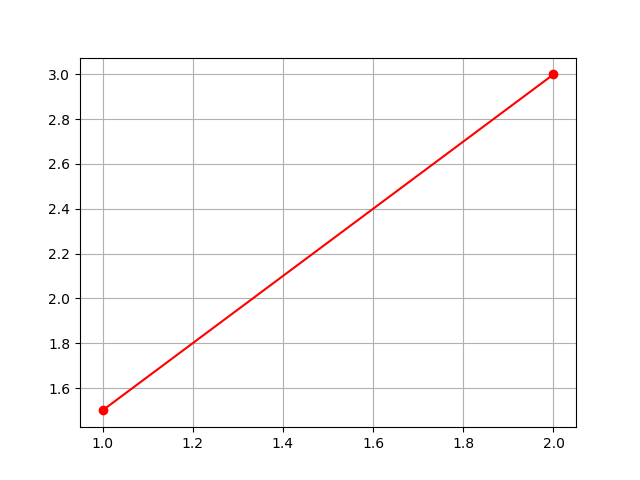
\includegraphics{sel101_1.png}
\end{figure}
Καλύτερα όμως είναι να βάλουμε και το σημείο (0,0) ως εξής:
\begin{lstlisting}
import matplotlib.pyplot as plt

plt.clf()
points = [(0,0),(1,1.5),(2,3)]

x = [p[0] for p in points]
y = [p[1] for p in points]

plt.grid()
plt.plot(x,y, marker='o', c='r')

plt.show()
\end{lstlisting}
\begin{figure}
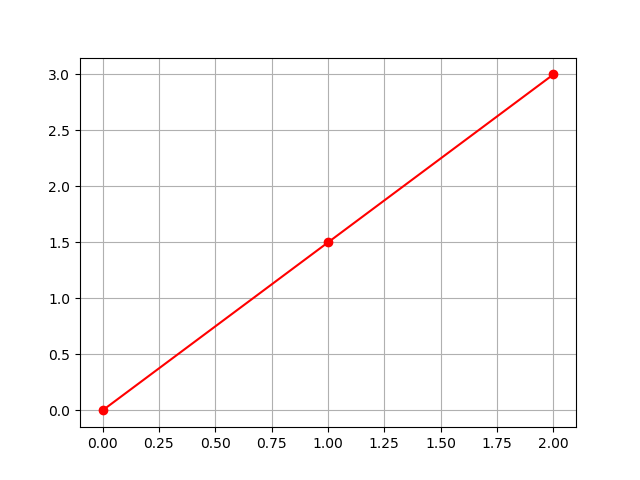
\includegraphics{sel101_1a.png}
\end{figure}

\begin{exercise}
\sel[2]{101}
Σε κατάλληλο ορθογώνιο σύστημα ημιαξόνων να σχεδιάσεις τις γραφικές παραστάσεις για κάθε μία από τις ακόλουθες σχέσεις αναλογίας: 

(α)	$y = \left(\frac{1}{2}\right)\cdot x$,	

(β)	$y = 3 \cdot x$,	

(γ)	$y =	5,5	\cdot x$

(δ)	$y =	10\cdot x$,	

(ε) $y  =	0,01 \cdot x$.
\end{exercise}

Μπορούμε να τις σχεδιάσουμε και όλες μαζί με διαφορετικά χρώματα. Έχουν ένα κοινό σημείο ενώ μπορούμε να υπολογίσουμε εύκολα ένα δεύτερο, π.χ. για $x=10$.
\begin{lstlisting}
import matplotlib.pyplot as plt
from sympy import *
x = symbols('x')

analogies = [1/2*x,3*x,5.5*x,10*x,0.01*x]
colors = ['r','g','b','c','m']
for (i,s) in enumerate(analogies):
    x = symbols('x')
    points = [(0,0),(10,s.subs(x,10))]
    x = [p[0] for p in points]
    y = [p[1] for p in points]
    plt.grid()
    plt.plot(x,y, marker='o', c=colors[i])

plt.show()
\end{lstlisting}
\begin{figure}
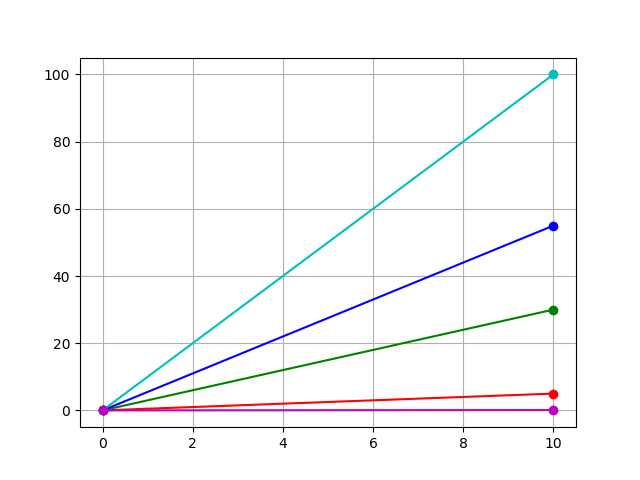
\includegraphics{sel101_2.png}
\end{figure}
Όμως τα συστήματα δεν είναι κατάλληλα για όλες τις γραφικές παραστάσεις ειδικά η τελευταία φαίνεται να είναι σταθερή στο 0. Αν τη σχεδιάσουμε μόνη της η matplotlib θα υπολογίσει ένα κατάλληλο σύστημα αξόνων, δες στον άξονα y.
\begin{lstlisting}
import matplotlib.pyplot as plt
from sympy import *

points = [(0,0),(10,0.01*10]
x = [p[0] for p in points]
y = [p[1] for p in points]
plt.grid()
plt.plot(x,y, marker='o', c='m')

plt.show()
\end{lstlisting}
\begin{figure}
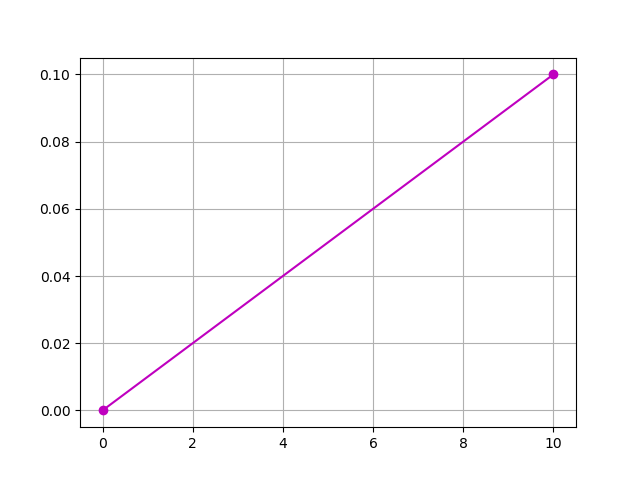
\includegraphics{sel101_2a.png}
\end{figure}

\begin{exercise}
Αντιστοίχισε	κάθε	πίνακα	με	ένα	από	τους	προτεινόμενους	τύπους:
\begin{table}
\begin{tabular}{cccc}
(A) & 
\begin{tabular}{|c|c|c|c|}
\hline
x&4&7&12\\\hline
y&10&17,5&30\\\hline
\end{tabular}
&(1)&$y=2x+3$\\
(B) & 
\begin{tabular}{|c|c|c|c|}
\hline
x&5&7,5&9\\\hline
y&11&16&19\\\hline
\end{tabular}
&(2)&$y=3x$\\
(Γ) & 
\begin{tabular}{|c|c|c|c|}
\hline
x&2&3&10\\\hline
y&7&9&23\\\hline
\end{tabular}
&(3)&$y=12:x$\\
(Δ) & 
\begin{tabular}{|c|c|c|c|}
\hline
x&2&4&6\\\hline
y&6&3&2\\\hline
\end{tabular}
&(4)&$y=2,5x$\\
(E) & 
\begin{tabular}{|c|c|c|c|}
\hline
x&2&5&0,5\\\hline
y&1&2,5&0,25\\\hline
\end{tabular}
&(5)&$y=2x+2$\\
(Z) & 
\begin{tabular}{|c|c|c|c|}
\hline
x&0,2&6&10\\\hline
y&2,4&14&22\\\hline
\end{tabular}
&(6)&$y=2x+1$\\
(H) & 
\begin{tabular}{|c|c|c|c|}
\hline
x&1&1,2&2,5\\\hline
y&3&3,6&7,5\\\hline
\end{tabular}
&(7)&$y=4x-1$\\
(Θ) & 
\begin{tabular}{|c|c|c|c|}
\hline
x&0,8&1&1,5\\\hline
y&2,2&3&5\\\hline
\end{tabular}
&(8)&$y=0,5x$\\
\end{tabular}
\end{table}
\end{exercise}
\begin{lstlisting}
from sympy import *
x = symbols('x')
pointsList = [[(4,10),(7,17.5),(12,30)],
              [(5,11),(7.5,16),(9,19)],
              [(2,7),(3,9),(10,23)],
              [(2,6),(4,3),(6,2)],
              [(2,1),(5,2.5),(0.5,0.25)],
              [(0.2,2.4),(6,14),(10,22)],
              [(1,3),(1.2,3.6),(2.5,7.5)],
              [(0.8,2.2),(1,3),(1.5,5)]]

typoi = [2*x+3,3*x,12/x,2.5*x,2*x+2,2*x+1,4*x-1,0.5*x]
onomataPinaka = ['Α','Β','Γ','Δ','Ε','Ζ','Η','Θ']

for (arithmosPinaka,points) in enumerate(pointsList):
    for (arithmosTipou, t) in enumerate(typoi):
        for p in points:
            x = symbols('x')
            if abs((p[1] - t.subs(x,p[0]))) > 1e-8:
                break
        else:
            print(onomataPinaka[arithmosPinaka],'-',arithmosTipou+1)
\end{lstlisting}

Που δίνει το αποτέλεσμα:

\begin{lstlisting}
Α - 4
Β - 6
Γ - 1
Δ - 3
Ε - 8
Ζ - 5
Η - 2
Θ - 7
\end{lstlisting}

Χρησιμοποιούμε abs((p[1] - t.subs(x,p[0]))) > 1e-8 αντί για το πιο απλό p[1]!=t.subs(x,p[0]) γιατί στην δεύτερη περίπτωση θα έχουμε σφάλματα απο στρογγυλοποιήσεις.

\begin{exercise}
\sel[4]{101}
Ένας καταστηματάρχης αθλητικών ειδών διαθέτει 12.000€ για να αγοράσει φόρμες γυμναστικής, μαγιό και αθλητικά παπούτσια. Κάθε φόρμα κοστίζει 40€ , κάθε μαγιό 20€ και κάθε ζευγάρι παπούτσια 50€. 

(α)  Να βρεις τις σχέσεις αναλογίας “χρήματα-κομμάτια από κάθε είδος” και να τις  παραστήσεις γραφικά στο ίδιο σύστημα ορθογωνίων αξόνων. 

(β)  Ο καταστηματάρχης αποφάσισε να διαθέσει το ίδιο ποσό, για κάθε είδος. Βρες  πόσα κομμάτια από κάθε είδος θα αγοράσει με τα χρήματα που διαθέτει,   χρησιμοποιώντας μόνο τη γραφική παράσταση των σχέσεων που δημιούργησες  στο πρώτο ερώτημα της άσκησης.
\end{exercise}
$$y = x/40$$
$$y = x/20$$
$$y = x/50$$

Αν δώσει 0 ευρώ τότε το y είναι 0 σε όλες τις γραφικές παραστάσεις. Αν δώσει 200 ευρώ τότε θα πάρει 5 φόρμες ($200/40=5$), 10 μαγιό ($200/40=10$), και 4 ζευγάρια αθλητικά παπούτσια ($200/50=40$).
Οπότε μπορούμε να σχεδιάσουμε τις ευθείες με τα σημεία: (0,0) και (200,5), (200,10), (200,50) αντίστοιχα. 
\begin{lstlisting}
import matplotlib.pyplot as plt

plt.clf()
pointslist = [[(0,0),(200,5)],
                        [(0,0),(200,10)],
                        [(0,0),(200,50]]
colors = ['r','g','b']
for (i,points) in enumerate(pointslist):
    x = [p[0] for p in points]
    y = [p[1] for p in points]
    plt.grid([10,10])
    plt.plot(x,y, marker='o', c=colors[i])

plt.show()
\end{lstlisting}

\begin{figure}
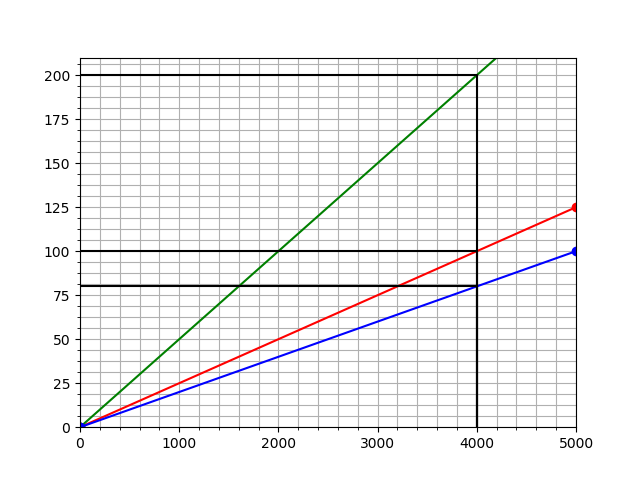
\includegraphics{sel101_4a.png}
\end{figure}
\begin{exercise}
\sel{103}
Για	να	φτιάξουμε	γλυκό	βύσσινο	πρέπει	να	καθαρίσουμε	τα	βύσσινα	από	τα	κουκούτσια.	Αν	καθαρίσουμε	2,5	Kg	βύσσινο,	παίρνουμε	2	Kg	καθαρό	βύσσινο. Αν	καθαρίσουμε	5	Kg	βύσσινο,	τι	ποσότητα	καθαρού	βύσσινου	θα	πάρουμε; 
\end{exercise}
Για αυτή την άσκηση και όλες τις αντίστοιχες μπορούμε να προγραμματίσουμε μια συνάρτηση:
\begin{lstlisting}
def analoga(gnwsto1,gnwsto2,analogo1):
    #analogo2/analogo1  = gnwsto2/gnwsto1
    analogo2 = gnwsto2/gnwsto1*analogo1
    return(analogo2)

print(analoga(2,5,2,5))
\end{lstlisting}
Που δίνει το σωστό αποτέλεσμα
\begin{lstlisting}
4.0
\end{lstlisting}
\begin{exercise}
\sel{104}
Ένας	μεσίτης	αγοράζει	ένα	σπίτι	360.000	€	και	σκοπεύει	να	το	πουλήσει	με	κέρδος	28\%.	Σε	έναν	πελάτη	έκανε	έκπτωση	15\%,	επί	της	τιμής	πώλησης. 

(α)		Πόσο	πουλήθηκε	το	σπίτι	στον	πελάτη	αυτόν; 

(β)		Ποιο	είναι	το	ποσοστό	κέρδους	του	μεσίτη,	για	το		σπίτι	αυτό; 
\end{exercise}
\begin{lstlisting}
>>> arxikiTimi = analoga(100,128,360000)
>>> arxikiTimi
460800.0
>>> telikiTimi = analoga(100,85,460800)
>>> telikiTimi
391680.0
>>> kerdos = (telikiTimi-360000)/360000*100
>>> kerdos
8.799999999999999
>>> 
\end{lstlisting}
Άρα λόγω της έκπτωσης το τελικό κέρδος του μεσίτη ήταν 8.8\%.
\begin{exercise}
\sel[1]{105}
Ένας	πάσσαλος	ύψους	1,2	m	ρίχνει	σκιά	3	m.	Την	ίδια	στιγμή	ένα	δέντρο	ρίχνει	σκιά	14	m.	Αν	γνωρίζουμε	ότι	τα	ποσά	ύψος	-	σκιά	είναι	ανάλογα,	να	βρεθεί	το	ύψος	του	δέντρου.
\end{exercise}
\begin{lstlisting}
>>> analoga(3,1.2,14)
5.6
\end{lstlisting}
\begin{exercise}
\sel{2}[105]
Το	βάρος	στο	φεγγάρι	και	το	βάρος	στη	γη	είναι	ποσά	ανάλογα.	Ένας	αστροναύτης	ζύγιζει	στο	φεγγάρι	12,9	Kg	και	στη	γη	78	Kg.	Πόσο	θα	ζυγίζει	στο	φεγγάρι	ένα	παιδί,	που 	στη	γη	έχει	βάρος	52	Kg;
\end{exercise}
\begin{lstlisting}
>>> analoga(78,12.9,52)
8.6
\end{lstlisting}
\begin{exercise}
\sel[3]{105}
Aπό	100	Kg	σταφύλια	βγαίνουν	80	Kg	μούστος.	Ένας	αμπελουργός	θέλει	να	γεμίσει	με	μούστο	6	βαρέλια,	των	350	Kg	το	καθένα.	Πόσα	K	σταφύλια,	της	ίδιας	ποιότητας,	πρέπει	να	πατήσει;
\end{exercise}
\begin{lstlisting}
>>> analoga(80,100,6*350)
2625.0
\end{lstlisting}
\begin{exercise}
\sel[4]{105}
Δύο	εργάτες	δούλεψαν	σε	μια	οικοδομή	και	πήραν	μαζί	270€ .	O	πρώτος	δούλεψε	4	ημέρες	και	ο	δεύτερος	5	ημέρες.	Πόσα	χρήματα	αντιστοιχούν	στον	καθένα.
\end{exercise}
\begin{lstlisting}
>>> analoga(9,270,4)
120.0
>>> analoga(9,270,5)
150.0
\end{lstlisting}
Και όντως $120+150=270$.
\begin{exercise}
\sel[5]{105}
Το	θαλασσινό	νερό	περιέχει	αλάτι	σε	ποσοστό	3\%.	Πόσα	κιλά	θαλασσινό	νερό	πρέπει	να	εξατμιστούν	για	να	πάρουμε	60Kg	αλάτι;
\end{exercise}
\begin{lstlisting}
>>> analoga(3,100,60)
2000.0000000000002
\end{lstlisting}
Άρα 2 τόνοι θαλασσινό νερό.
\begin{exercise}
\sel[6]{105}
Ένας	γεωργός	είχε	ένα	χωράφι	7	στρέμματα	και	πήρε	και	το	γειτονικό	χωράφι	εμβαδού	8	στρεμμάτων,	για	να	φυτέψει	καλαμπόκι.	Η	συμφωνία	με	το	γείτονά	του	ήταν	να	του	δώσει	το	15	της	παραγωγής	του	χωραφιού	του.	Η	συνολική	παραγωγή	ήταν	14	τόνοι	καλαμπόκι.	Πόσους	τόνους	θα	πάρει	ο	γεωργός	και	πόσους	ο	γείτονάς	του;
\end{exercise}
\begin{lstlisting}
>>> xwrafi8 = analoga(7+8,14000,8)
>>> analoga(100,15,xwrafi8)
1120.0
\end{lstlisting}
\begin{exercise}
\sel[7]{105}
Αν	ψήσουμε	2,5	Κ	ωμό	κρέας	θα	μείνει	1,9	K	ψημένο	κρέας. (α)		Πόσο	είναι	το	ποσοστό	απώλειας	που	έχουμε; (β)		Πόσο	κρέας	πρέπει	να	ψήσουμε	για	να	έχουμε	2,3	K	ψημένο	κρέας;
\end{exercise}
\begin{lstlisting}
>>> analoga(2.5,2.5-1.9,100)
24.000000000000004
>>> analoga(1.9,2.5,2.3)
3.026315789473684
\end{lstlisting}
Άρα 3Kg ωμό κρέας.
\begin{exercise}
\sel[8]{105}Η	μηνιαία	κάρτα	απεριορίστων	διαδρομών	στοιχίζει	12	Q	και	η	τιμή	της	θα	αυξηθεί,	κατά	75.	Το	εισιτήριο	στο	αστικό	λεωφορείο	είναι	0,7	Q	και	θα	αυξηθεί,	κατά	50.	Ένας	εργαζόμενος	παίρνει	λεωφορείο,	για	να	πάει	και	να	γυρίσει	από	τη	δουλειά	του	κάθε	ημέρα,	για	είκοσι	φορές	το	μήνα.	Τον	συμφέρει	η	χρήση	της	κάρτας	ή	όχι;
\end{exercise}
Το κόστος της κάρτας θα είναι:
\begin{lstlisting}
>>> analoga(100,175,12)
21.0
\end{lstlisting}
Το κόστος του εισιτηρίου θα είναι:
\begin{lstlisting}
>>> analoga(100,150,0.7)
1.0499999999999998
\end{lstlisting}
1.05€
και το κόστος των 20 εισιτηρίων θα είναι:
\begin{lstlisting}
>>> 20*1.05
21.0
\end{lstlisting}
Άρα ίδιο κόστος με αυτό της κάρτας.

\begin{exercise}
\sel[9]{105}Ένα	κεφάλαιο	δίνει	τόκο	1.000	Q	το	χρόνο,	με	επιτόκιο	10.	Αν	το	επιτόκιο	μειωθεί	κατά	20,	πόσο	τοις	εκατό	πρέπει	ν’	αυξήσουμε	το	κεφάλαιό	μας	για	να	έχουμε	τον	ίδιο	τόκο,	παρά	τη	μείωση	του	επιτοκίου;
\end{exercise}
Το αρχικό κεφάλαιο είναι:
\begin{lstlisting}
>>> analoga(10,100,1000)
10000.0
\end{lstlisting}
Το νέο επιτόκιο είναι:
\begin{lstlisting}
>>> analoga(100,80,10)
8.0
\end{lstlisting}
Οπότε το νέο κεφάλαιο θα πρέπει να είναι:
\begin{lstlisting}
>>> analoga(8,100,1000)
12500.0
\end{lstlisting}
και το ποσοστό αύξησης του κεφαλαίο θα είναι:
\begin{lstlisting}
>>> analoga(10000,2500,100)
25.0
\end{lstlisting}
\begin{exercise}
\sel[10]{105} Συμπλήρωσε	τον	παρακάτω	πίνακα	και	σχεδίασε	διάγραμμα	που	αντιστοιχεί	στα	δεδομένα	του	προβλήματος.
\begin{table}
\begin{tabular}{|c|c|c|c|c|c|c|c|}\hline
 &ΣΥΝΟΛΟ & Με 0 παιδιά & Με 1 παιδί & Με 2 παιδιά & Με 3 παιδιά & Με 4 παιδιά & Πάνω από 5 παιδιά     \\\hline
Οικογένειες &200 & 10 & 40 & 80 & 50 & 15 & 5     \\\hline
Ποσοστά & 100\%& &  &  & &  &     \\\hline
\end{tabular}
\end{table}
\end{exercise}
\begin{lstlisting}
>>> analoga(200,10,100)
5.0
>>> analoga(200,40,100)
20.0
>>> analoga(200,80,100)
40.0
>>> analoga(200,50,100)
25.0
>>> analoga(200,15,100)
7.5
>>> analoga(200,5,100)
2.5
\end{lstlisting}
και ο πίνακας γίνεται:
\begin{table}
\begin{tabular}{|c|c|c|c|c|c|c|c|}\hline
 &ΣΥΝΟΛΟ & Με 0 παιδιά & Με 1 παιδί & Με 2 παιδιά & Με 3 παιδιά & Με 4 παιδιά & Πάνω από 5 παιδιά     \\\hline
Οικογένειες &200 & 10 & 40 & 80 & 50 & 15 & 5     \\\hline
Ποσοστά & 100\%&5 & 20 &40  &25 &7.5  & 2.5    \\\hline
\end{tabular}
\end{table}
Μια επαλήθευση δίνει:
\begin{lstlisting}
>>> 5 + 20 +40  +25 +7.5  + 2.5   
100.0
\end{lstlisting}
\section{Αντιστρόφως ανάλογα ποσά}
\begin{exercise}
\sel{106}
Ξεκινούν ταυτόχρονα από μια πόλη:  
(α)  ένα αυτοκίνητο που τρέχει με ταχύτητα 120 kmh  

(β)  ένα αεροπλάνο με 600 Kmh  

(γ)  μία μοτοσικλέτα με 75 Kmh  

(δ)  ένα λεωφορείο που τρέχει με 80 Kmh  

(ε)  ένα ελικόπτερο με 300 Kmh 

(στ)  ένα ταξί με 100 Kmh  

(ζ)  μία βέσπα με 60 Kmh και  

(η)  ένα πούλμαν με 90 Kmh

To τέλος της διαδρομής είναι μια άλλη πόλη, που απέχει 600 Km.
\begin{itemize}
 \item Βρες σε πόσες ώρες, θα φθάσει το καθένα στον προορισμό του και συμπλήρωσε  τον παρακάτω πίνακα:
 \begin{table}
 \begin{tabular}{|c|c|c|c|c|c|c|c|c|}
 Ταχύτητα σε Km/h&&&&&&&&\\\hline
 Χρόνος σε ώρες&&&&&&&&\\\hline
 \end{tabular}
 \end{table}
 \item Ποια σχέση συνδέει τα μεγέθη της ταχύτητας και του χρόνου;
 \item Toποθέτησε τα ζεύγη των τιμών που βρήκες, σε ένα σύστημα ημιαξόνων και  ένωσε τα σημεία, που ορίζουν τα ζεύγη αυτά, με μία γραμμή. Τι παρατηρείς;
\end{itemize}
\end{exercise}
\begin{lstlisting}
>>> 600/120
5.0
>>> 600/600
1.0
>>> 600/75
8.0
>>> 600/80
7.5
>>> 600/300
2.0
>>> 600/100
6.0
>>> 600/60
10.0
>>> 600/90
6.666666666666667
\end{lstlisting}
Οπότε ο πίνακας γίνεται:
\begin{table}
 \begin{tabular}{|c|c|c|c|c|c|c|c|c|}
 Ταχύτητα σε Km/h&120&600&75&80&300&100&60&90\\\hline
 Χρόνος σε ώρες&5&1&8&7.5&2&6&10&6,66\\\hline
 \end{tabular}
 \end{table}

Τα ποσά είναι αντιστρόφως ανάλογα.

\begin{lstlisting}
import matplotlib.pyplot as plt

plt.clf()
points = [(120,5), (600,1), (75,8), (80,7.5), (300,2), (100,6), (60,10), (90,6.66)]
x = [p[0] for p in points]
y = [p[1] for p in points]
color=['m','g','r','b','c']
plt.grid()
plt.scatter(x,y, s=100 ,marker='o', c=color)

plt.show()
\end{lstlisting}
\begin{figure}
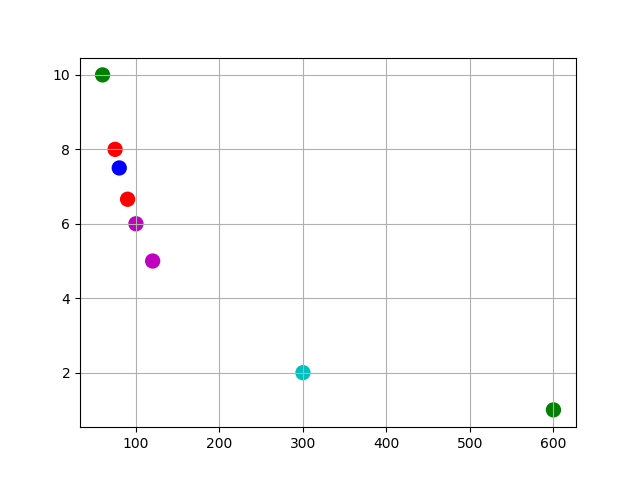
\includegraphics{graph4.png}
\caption{Χρόνος ως προς την ταχύτητα}
\end{figure}
\begin{exercise}
\sel{106}
Ένα συνεργείο που αποτελείται από 8 εργάτες χρειάζεται 30 ημέρες για να ολοκληρώσει ένα οικοδομικό έργο. 
\begin{itemize}
	\item  Πόσες ημέρες θα χρειαστεί το συνεργείο,  που αποτελείται από 2, 4, 6, 10, 12, 24 ή 48  εργάτες για να τελειώσει το ίδιο έργο;
	\item Μπορείς να συμπληρώσεις τον παρακάτω  πίνακα;
	\begin{table}
	\begin{tabular}{|c|c|c|c|c|c|c|c|c|}\hline
	Εργάτες συνεργείου &2    & 4& 6& 8& 10& 12& 24& 48\\\hline
	Ημέρες εργασίας       & &    &   & 30 & & & & \\\hline
	\end{tabular}
	\end{table}
\item  Τι παρατηρείς για το γινόμενο ``εργάτες'' $\cdot$ ``ημέρες'';
\item  Τοποθέτησε τα ζεύγη των τιμών του πίνακα, σε ένα σύστημα ημιαξόνων και  ένωσε τα σημεία, που ορίζουν τα ζεύγη αυτά, με μία γραμμή. Τι παρατηρείς;
\end{itemize}
\end{exercise} 
\begin{lstlisting}
>>> 8/2*30
120.0
>>> 8/4*30
60.0
>>> 8/6*30
40.0
>>> 8/8*30
30.0
>>> 8/10*30
24.0
>>> 8/12*30
20.0
>>> 8/24*30
10.0
>>> 8/48*30
5.0
>>>
\end{lstlisting}
Ο πίνακας γίνεται:
	\begin{table}
	\begin{tabular}{|c|c|c|c|c|c|c|c|c|}\hline
	Εργάτες συνεργείου &2    & 4 & 6& 8& 10& 12& 24& 48\\\hline
	Ημέρες εργασίας       &120 &60& 40   & 30 &24 & 20&10 &5 \\\hline
	\end{tabular}
	\end{table}

\begin{lstlisting}
>>> erg = [2,4,6,8,10,12,24,48]
>>> mer = [120,60,40,30,24,20,10,5]
>>> for i in range(8):
...     print(erg[i]*mer[i])
...
240
240
240
240
240
240
240
240
\end{lstlisting}
Το γινόμενο είναι πάντα 240.
\begin{lstlisting}
import matplotlib.pyplot as plt

plt.clf()
points = [(1,120),(4,60),(6,40),(8,30),(10,24),(12,20),(24,10),(48,5)]
x = [p[0] for p in points]
y = [p[1] for p in points]
color=['m','g','r','b','c']
plt.grid()
plt.scatter(x,y, s=100 ,marker='o', c=color)

plt.show()
\end{lstlisting}
\begin{figure}
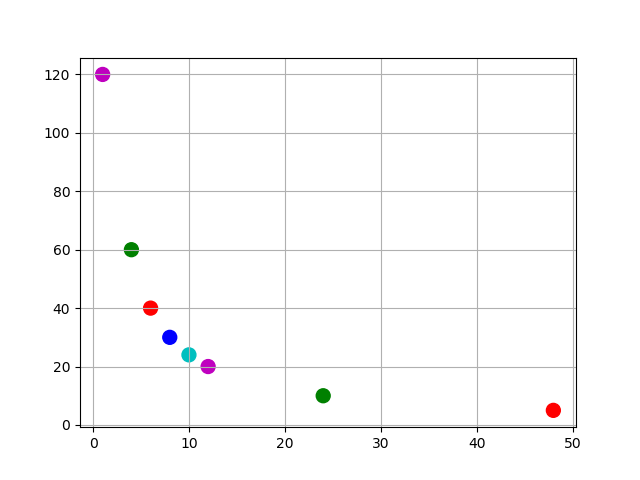
\includegraphics{graph5.png}
\end{figure}
\begin{exercise}
\sel{107}

Ένα ορθογώνιο παραλληλόγραμμο έχει διαστάσεις x και y. Aν γνωρίζεις ότι το εμβαδόν του ορθογωνίου είναι 144 m2, μπορείς να βρεις δεκατέσσερις ακέραιες τιμές των διαστάσεών του και να συμπληρώσεις τον παρακάτω πίνακα;
\begin{table}
\begin{tabular}{|c|c|c|c|c|c|c|c|c|c|c|c|c|c|c|}\hline
x & 1 & 2 & 3 &  4 & 6 & 12 & 18 & 20 & 22 & 24 & 30 &  32 & 34 & 36 \\\hline
y & & & & & & & & & & & & & &  \\\hline
\end{tabular}
\end{table}
\begin{itemize}
\item  Ποια σχέση συνδέει τις διαστάσεις του ορθογωνίου με το εμβαδόν του;
\item Τοποθέτησε τα ζεύγη των τιμών του πίνακα, σε ένα σύστημα ημιαξόνων και  ένωσε τα σημεία, που ορίζουν τα ζεύγη αυτά, με μία γραμμή. Τι παρατηρείς;
\item Ποιο ορθογώνιο, απ’ αυτά που βρήκες, έχει τη μικρότερη περίμετρο;
\end{itemize}
\end{exercise}
\begin{lstlisting}
>>> 144/1
144.0
>>> 144/2
72.0
>>> 144/3
48.0
>>> 144/4
36.0
>>> 144/6
24.0
>>> 144/12
12.0
>>> 144/18
8.0
>>> 144/20
7.2
>>> 144/22
6.545454545454546
>>> 144/24
6.0
>>> 144/30
4.8
>>> 144/32
4.5
>>> 144/34
4.235294117647059
>>> 144/36
4.0
\end{lstlisting}
\begin{table}
\begin{tabular}{|c|c|c|c|c|c|c|c|c|c|c|c|c|c|c|}\hline
x & 1 & 2 & 3 &  4 & 6 & 12 & 18 & 20 & 22 & 24 & 30 &  32 & 34 & 36 \\\hline
y &144&72&48&36&24&12&8&7.2&6.55&6&4.8&4.5&4,235&4 \\\hline
\end{tabular}
\end{table}

\begin{lstlisting}
import matplotlib.pyplot as plt

plt.clf()
x = [1,2,3,4,6,12,18,20,22,24,30,32,34,36]
y = [144/p for p in x]
plt.grid()
plt.scatter(x,y, s=100 ,marker='.', c='m')

plt.show()
\end{lstlisting}

\begin{figure}
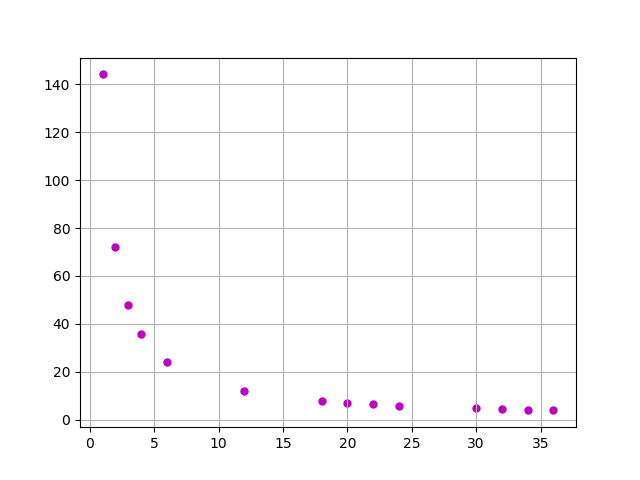
\includegraphics{graph6.png}
\end{figure}
Για την περίμετρο μπορούμε να κάνουμε μια γραφική παράσταση για τα σημεία που έχουμε:
\begin{lstlisting}
import matplotlib.pyplot as plt

plt.clf()
x = [1,2,3,4,6,12,18,20,22,24,30,32,34,36]
y = [144/p for p in x]
perimetros = [2*p+2*144/p for p in x]
plt.grid()
plt.scatter(x,y, s=100 ,marker='.', c='m')
plt.scatter(x,perimetros,s=100,marker='.',c='r')
plt.show()
\end{lstlisting}
\begin{figure}
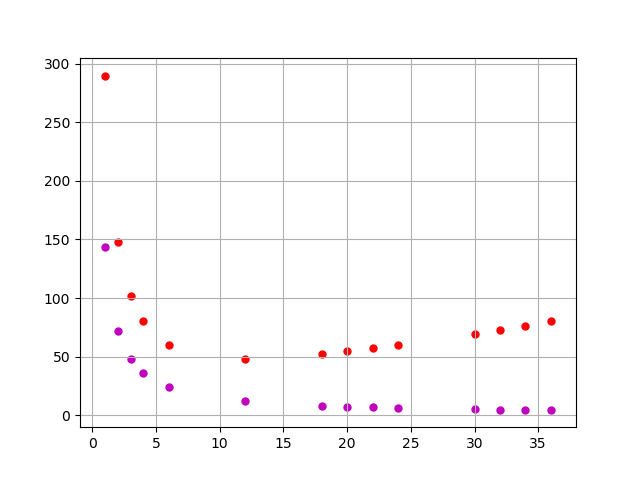
\includegraphics{graph7.png}
\end{figure}

Βλέπουμε ότι η μικρότερη περίμετρος προκύπτει όταν το x είναι 12.


Για την ακρίβεια μπορούμε να δούμε τη γραφική παράσταση για πολλά σημεία ως εξής:
\begin{lstlisting}
import matplotlib.pyplot as plt
from numpy import arange

plt.clf()
x = arange(1,20,0.5)
y = [144/p for p in x]
perimetros = [2*p+2*144/p for p in x]
plt.grid()
plt.scatter(x,y, s=100 ,marker='.', c='m')
plt.scatter(x,perimetros,s=100,marker='.',c='r')
plt.show()
\end{lstlisting}
\begin{figure}
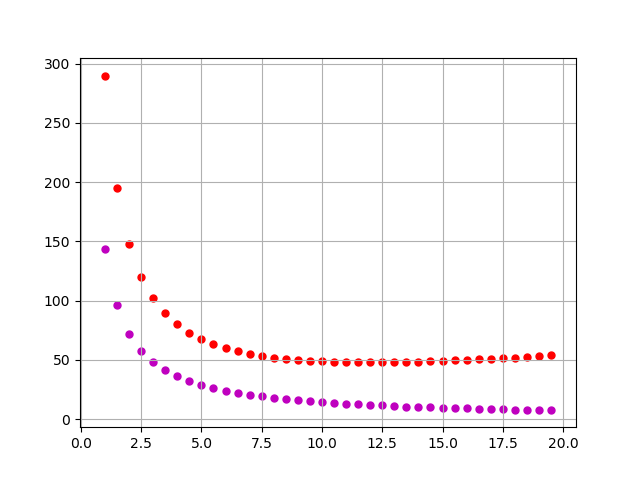
\includegraphics{graph8.png}
\end{figure}
\begin{exercise}
\sel{108}
Ένας ελαιοπαραγωγός χρησιμοποιεί δοχεία των 20 lt, 15 lt, 10 lt και 5 lt, για να συσκευάσει το λάδι που παράγει. Η παραγωγή του είναι 3.600 lt. Θέλει να συσκευάσει την ίδια ποσότητα λαδιού σε κάθε μία από τις τέσσερις διαφορετικές συσκευασίες. (α)  Πόσα δοχεία χρειάζεται από κάθε είδος; (β)  Πόσο θα κοστίσει η συσκευασία της παραγωγής του αν στοιχίζει 0,4€ το δοχείο  των 20 lt, 0,3€ το δοχείο των 15 lt,  0,2€ το δοχείο των 10 lt και 0,1€ το δοχείο  των 5 lt; 
\end{exercise}
\begin{lstlisting}
posotita = 3600/4
x = [20,15,10,5]
y = []
for doxeio in x:
    plithos = posotita / doxeio
    y.append(plithos)

kostos = [0.4,0.3,0.2,0.1]
synolikoKostos = 0
for (i,p) in enumerate(y):
    synolikoKostos += kostos[i]*p

print(plithos)
print(kostos)
\end{lstlisting}
που δίνει αποτέλεσμα
\begin{lstlisting}
[45.0, 60.0, 90.0, 180.0]
72.0
\end{lstlisting}
Δηλαδή 45 δοχεία των 20lt, 60 δοχεία των 15lt, 90 δοχεία των 10lt και 180 δοχεία των 5lt. Το συνολικό κόστος για τα δοχεία έιναι 72€.
\begin{exercise}
\sel{109}
Εξέτασε τους παρακάτω πίνακες:

α)

\begin{table}
\begin{tabular}{|c|c|c|c|c|}
x&1&2&3&4\\\hline
y&2&1&$\frac{2}{3}$&$\frac{1}{2}$\\\hline
\end{tabular}
\end{table}

β)

\begin{table}
\begin{tabular}{|c|c|c|c|}
x&0,25&0,4&0,5\\\hline
y&10&6,25&5\\\hline
\end{tabular}
\end{table}

γ)

\begin{table}
\begin{tabular}{|c|c|c|c|c|}
x&$\frac{1}{100}$&$\frac{2}{58}$&$\frac{7}{10}$&4\\\hline
y&100&29&$\frac{10}{7}$&$\frac{1}{4}$\\\hline
\end{tabular}
\end{table}

δ)

\begin{table}
\begin{tabular}{|c|c|c|c|}
x&3&6&9\\\hline
y&9&5&3\\\hline
\end{tabular}
\end{table}

\end{exercise}
\sel[3]{109}
Θα φτιάξουμε μια συνάρτηση που να παίρνει σαν εισόδους δύο πίνακες με τιμές x και y και θα δίνει σαν αποτέλεσμα αν αυτές οι τιμές είναι αντιστρόφως ανάλογες ή όχι. Θα βασιστεί στο ότι αν τα ποσά είναι αντιστρόφως ανάλογα το γινόμενό τους είναι πάντα το ίδιο.
\begin{lstlisting}
def antistrofosanaloga(x,y):
    if len(x) != len(y):
        print('Τα δεδομένα δεν έχουν το ίδιο μέγεθος')
        return(None)
    ginomeno = x[0]*y[0]
    for i in range(len(x)):
        if x[i]*y[i]!=ginomeno:
            return(False)
    return(True)

print(antistrofosanaloga([1,2,3,4],[2,1,2/3,1/2]))
print(antistrofosanaloga([0.25,0.4,0.5],[10,6.25,5]))
print(antistrofosanaloga([1/100,2/58,7/10,4],[100,29,10/7,1/4]))
print(antistrofosanaloga([3,6,9],[9,5,3]))
\end{lstlisting}
που δίνει αποτέλεσμα
\begin{lstlisting}
True
True
True
False
\end{lstlisting}
Άρα οι πίνακες α,β,γ έχουν ποσά αντιστρόφως ανάλογα ενώ ο πίνακας δ όχι.
\begin{exercise}
\sel[4]{109}
Τα ποσά x και  είναι αντιστρόφως ανάλογα. 
(α) Συμπλήρωσε τον πίνακα: 

\begin{table}
\begin{tabular}{|c|c|c|c|c|c|c|c|c|c|c|c|}\hline
x&0,2&0,5&0,7&1      &      &      & 2,3&3&            &10&12\\\hline
y&       &     &      & 3,5 &2,5&1,75&      &   &0,875&     &\\\hline
\end{tabular}
\end{table}

(β)  Βρες τα σημεία που παριστάνουν κάθε ζευγάρι τιμών (x, ), σε κατάλληλο  σύστημα ορθογωνίων ημιαξόνων και σχεδίασε την 
υπερβολή. 
\end{exercise}
\begin{lstlisting}
>>> 3.5/0.2
17.5
>>> 3.5/0.5
7.0
>>> 3.5/0.7
5.0
>>> 3.5/2.5
1.4
>>> 3.5/1.75
2.0
>>> 3.5/2.3
1.5217391304347827
>>> 3.5/3
1.1666666666666667
>>> 3.5/0.875
4.0
>>> 3.5/10
0.35
>>> 3.5/12
0.2916666666666667
\end{lstlisting}

\begin{table}
\begin{tabular}{|c|c|c|c|c|c|c|c|c|c|c|c|}\hline
x&0,2 &0,5&0,7&1      &1,4& 2   & 2,3  &3        &4        &10   &12\\\hline
y&17,5&7    & 5  & 3,5 &2,5&1,75&1,52& 1,167&0,875&0,35 &0,29\\\hline
\end{tabular}
\end{table}

Για να σχεδιάσουμε φτιάχνουμε το πρόγραμμα:
\begin{lstlisting}
import matplotlib.pyplot as plt

plt.clf()
x=[0.2,0.5,0.7,1,1.4,2,2.3,3,4,10,12]
y=[17.5,7,5,3.5,2.5,1.75,1.52,1.167,0.875,0.35,0.29]
plt.grid()
plt.scatter(x,y, s=100 ,marker='.', c='m')
plt.show()
\end{lstlisting}
που δίνει το αποτέλεσμα
\begin{figure}
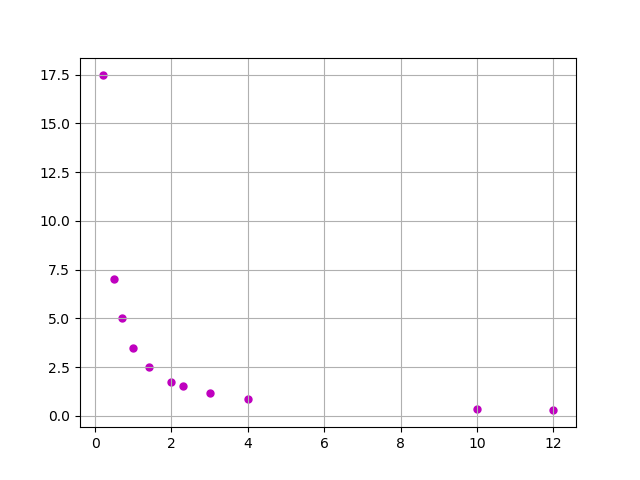
\includegraphics{graph9.png}
\end{figure}
\begin{exercise}
\sel[5]{109}
Για την αναδάσωση μιας πλαγιάς, εργάστηκαν 20 εργάτες για 10 ημέρες. Πόσοι εργάτες, ίδιας απόδοσης, χρειάζονται για να αναδασώσουν την έκταση αυτή, σε 8 ημέρες; 
\end{exercise}
Το γινόμενο εργάτες $\cdot$ ημέρες θα είναι σταθερό οπότε 
$$x\cdot 8 = 20\cdot 10$$
$$x = \frac{20\cdot 10}{8}$$
$$x =  25$$

\begin{lstlisting}
>>> 20*10/8
25.0
\end{lstlisting}
\begin{exercise}
\sel[6]{109}
Σε ένα αγρόκτημα, τοποθέτησαν ντομάτες σε 50 καφάσια, των 12 Kg το καθένα. Πόσα καφάσια των 20 kg θα χρειαζόντουσαν για να τοποθετήσουν τις ντομάτες. Αν κάθε καφάσι των 12 kg στοιχίζει 0,28€ και κάθε καφάσι των 20Kg 0,46€, ποια συσκευασία τους συμφέρει, ώστε να ελαχιστοποιηθεί το κόστος συσκευασίας του προϊόντος τους; 
\end{exercise}
\begin{lstlisting}
>>> ntomates = 50*12
>>> kafasia20 = ntomates/20
>>> kafasia20
30.0
>>> kostos12 = 50*0.28
>>> kostos12
14.000000000000002
>>> kostos20 = kafasia20*0.46
>>> kostos20
13.8
\end{lstlisting}
\begin{exercise}
\sel[8]{109}
Το πετρέλαιο που υπάρχει στη δεξαμενή μιας πολυκατοικίας, επαρκεί για 30 ημέρες, όταν καταναλώνονται 80 lt την ημέρα. Όταν το κρύο δυναμώνει, η ημερήσια κατανάλωση αυξάνεται, κατά 20\%. Για πόσες ημέρες θα φτάσει το πετρέλαιο;
\end{exercise}
\begin{lstlisting}
>>> neakatan = 80+80*20/100
>>> neakatan
96.0
>>> meres = 80*30/neakatan
>>> meres
25.0
\end{lstlisting}
\begin{exercise}
\sel[6]{112}
Συμπλήρωσε	τον	διπλανό	πίνακα	ανάλογων ποσών
\begin{table}
\begin{tabular}{|c|c|c|c|c|c|}
x&2&4 &  &12&16\\\hline
y&  &15&30& &\\hline
\end{tabular}
\end{table}
\end{exercise}
\begin{lstlisting}
>>> l = 15/4
>>> 2*l
7.5
>>> 30/l
8.0
>>> 12*l
45.0
>>> 16*l
60.0
\end{lstlisting}
\begin{table}
\begin{tabular}{|c|c|c|c|c|c|}
x&2   &4  &8 &12&16\\\hline
y&7.5&15&30&45 &60\\hline
\end{tabular}
\end{table}
\begin{exercise}
\sel[8]{112}
Συμπλήρωσε τον πίνακα των αντιστρόφως ανάλογων ποσών.
\begin{table}
\begin{tabular}{|c|c|c|c|c|c|}
x& 2&&&4&8\\\hline
y& 8&16&32&&\\\hline
\end{tabular}
\end{table}
\end{exercise}
\begin{lstlisting}
>>> gin = 2*8
>>> gin/16
1.0
>>> gin/32
0.5
>>> gin/4
4.0
>>> gin/8
2.0
\end{lstlisting}
\begin{table}
\begin{tabular}{|c|c|c|c|c|c|}
x& 2&  1&0.5&4&8\\\hline
y& 8&16&32&4&2\\\hline
\end{tabular}
\end{table}
